\chapter{Padrões, Metodologias e Tecnologias}

Neste capítulo, apresentam-se os padrões, metodologias e tecnologias utilizados para a realização deste trabalho. Para isto, demostra-se cada abordagem, seja ela aplicada na gerência do projeto ou no desenvolvimento da ferramenta de argumentação.    

\section{Scrum}
\label{scrum_met}

Desde o início dos anos 90, o Scrum vem sendo utilizado para gerenciar o desenvolvimento de produtos complexos. Segundo \cite{guiascrum} o Scrum é um framework estrutural que, a partir de regras bem definidas, permite a construção de produtos com alto valor de uma maneira produtiva e criativa. As regras do Scrum são dispostas em um processo iterativo e incremental. Apresenta-se na Figura \ref{scrum-estrutura} a estrutura geral do Scrum.

\graphicspath{{figuras/}}
\begin{figure}[H]
\centering
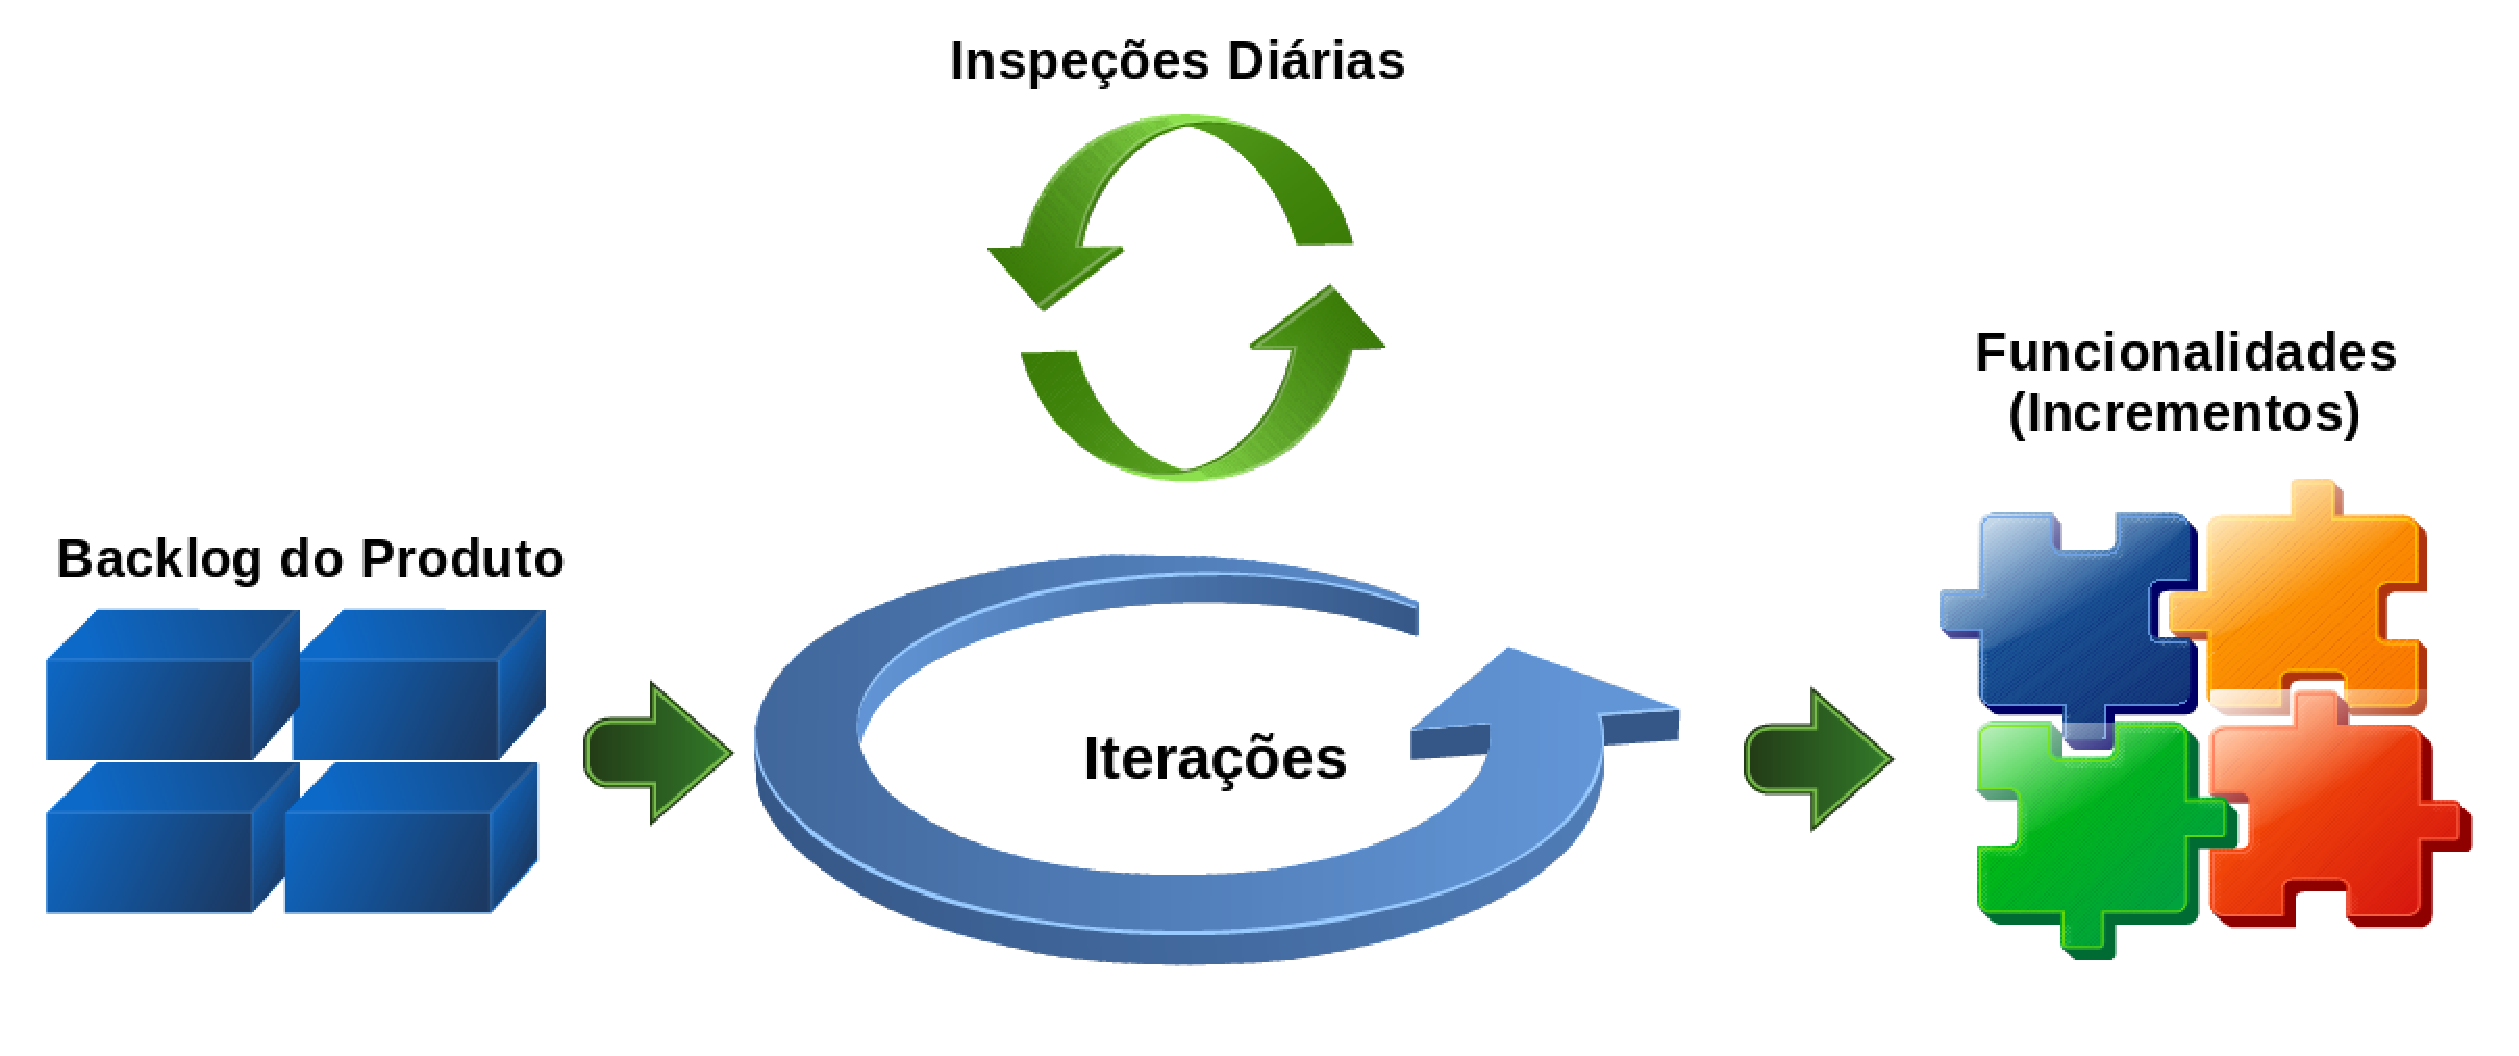
\includegraphics[width=0.9\textwidth]{scrum-estrutura}
\caption{Estrutura do Framework Scrum.}{Adaptado de \cite{schwaber2004}} 
\label{scrum-estrutura}
\end{figure}

A estrutura apresentada na Figura \ref{scrum-estrutura} funciona da seguinte forma. O laço inferior representa uma iteração contendo atividades de desenvolvimento. Esta iteração, também conhecida com \textit{Sprint}, tem como entrada os requisitos presentes no \textit{backlog} do produto. Durante a iteração, aconselha-se a ocorrência de reuniões diárias para que cada indivíduo da equipe possa inspecionar as atividades de seus companheiros. Ao término da iteração, um incremento do produto final é desenvolvido. Permitindo aos usuários chaves a chance de avaliar a funcionalidade e sugerir melhorias para o projeto.

Os times do Scrum são entidades auto-organizáveis e multifuncionais. A equipe deve escolher qual a melhor maneira de realizar seu trabalho. Para concluir suas pendências, exigi-se da equipe as competências necessárias sem depender de terceiros que não participam da equipe. O time é dividido da seguinte forma:

\begin{itemize}
\item \textit{Product Owner}: Possui conhecimento acerca do contexto da aplicação. Seu principal papel é agregar valor ao negócio. Para isto, realiza o gerenciamento do \textit{backlog} do produto, adicionando e priorizando requisitos.
\item Equipe de Desenvolvimento: Profissionais que implementam os requisitos contidos no \textit{backlog} do produto. Seu principal papel é entregar uma versão funcional do produto.
\item \textit{Scrum Master}: Remove possíveis impedimentos que poderiam prejudicar a execução do projetos. Possui papel de facilitador, aplicando as regras do Scrum de forma correta.  
\end{itemize}

O Scrum define uma série de eventos \textit{time-boxed} com o objetivo de criar uma simples rotina a ser seguida. Os eventos possuem uma duração máxima, porém, caso o objetivo do evento tenha sido concluído, ele pode ser finalizado previamente. Apresenta-se na Tabela \ref{tabela-scrum} a descrição dos principais eventos.

\begin{longtable}{|p{7cm}|p{7cm}|}
\caption{Eventos do Scrum.}\\
\hline
\textbf{Evento} & \textbf{Descrição} \\
\hline
\endfirsthead
\multicolumn{2}{c}%
{\tablename\ \thetable\ -- \textit{Continuação da Página Anterior}} \\
\hline
\textbf{Evento} & \textbf{Descrição} \\
\hline
\endhead
\hline \multicolumn{2}{r}{\textit{Continua na Próxima Página}} \\
\endfoot
\hline
\endlastfoot
Iteração (\textit{Sprint}) & Possui duração de aproximadamente um mês, em que uma versão funcional do produto é desenvolvida. Ao término de uma iteração, inicia-se outra. A iteração é composta de reunião de planejamento, encontros diários, implementação dos requisitos, revisão e retrospectiva da \textit{Sprint}. \\ \hline
Reunião Diária & Possui duração de aproximadamente 15 minutos. O papel deste evento é permitir que a equipe avalie  as atividades realizadas bem como a determinação de metas a serem concluídas até a próxima reunião diária. \\ \hline
Revisão da \textit{Sprint} & Possui duração de aproximadamente 4 horas. Ao término da \textit{Sprint}, o incremento desenvolvido deve ser inspecionado para verificar sua conformidade com o \textit{backlog} do produto. Durante a reunião de revisão, sugestões para otimizar o valor do produto são realizadas. \\ \hline  
Retrospectiva da \textit{Sprint} & Possui duração de aproximadamente 3 horas. Este evento representa uma oportunidade para a equipe identificar melhorias a serem aplicadas em \textit{Sprints} futuras. Para isto, é feita uma reflexão acerca dos pontos positivos e negativos da \textit{Sprint} avaliada.    
\label{tabela-scrum}
\end{longtable}

Além dos eventos, o Scrum contem alguns artefatos. O \textbf{\textit{backlog} do produto} representa uma lista contendo todos os requisitos que devem ser implementado. Geralmente os requisitos são descritos por meio de histórias de usuários. A lista pode sofrer mudanças a qualquer momento e reflete a visão que o \textit{Product Owner} possui do negócio. O \textbf{\textit{backlog} da \textit{Sprint}} é uma lista de itens que foram selecionados com base no \textit{backlog} do produto. Esta lista representa o trabalho a ser feito na \textit{Sprint}.     

Apesar de possuir uma difícil implantação, o Scrum se mostrou extremamente eficaz quando adotado corretamente. \cite{phamscrum2012} indica quatro vantagens obtidas com a adoção do Scrum:

\begin{itemize}

\item Mecanismos sistemáticos para a redução dos riscos: Através da inspeção freqüente e dos ciclos adaptativos o Scrum mitiga, com antecedência, possíveis inconsistências que poderiam dificultar a execução do projeto.

\item Ciclo de desenvolvimento de software sucinto: Por meio de iterações curtas, a equipe de desenvolvimento implementa versões incrementais do produto. Cada iteração dura aproximadamente um mês e pode compreender atividades de todo o processo de desenvolvimento de software.

\item Processo de gerenciamento de projetos adaptativo: As mudanças são vistas como oportunidades para melhorar. Ao término de cada iteração, reuniões para identificar inconsistências são realizadas. As lições aprendidas são aplicadas na definição de novas iterações.

\item Abordagem baseada na motivação e satisfação das pessoas: Seguindo os princípios da metodologia ágil, o objetivo é permitir que a equipe decida quais ações tomar para cumprir com a meta definida.      

\end{itemize}
      

\section{Engenharia de Requisitos: Orientação à Meta}
\label{meta_orient}

Os sistemas de informação estão cada vez mais inclusos no cotidiano das pessoas. Um fator a ser considerado no desenvolvimento de software é o ambiente no qual ele operará. A partir desta informação, aspectos sociais baseados no público alvo, condições de uso e restrições do software podem ser identificados. Modelos de desenvolvimento de software tradicionais pecam na inclusão destes aspectos sociais. Isto acaba diminuindo a aceitação do software pelos \textit{stackholders} \cite{borgida2009}.

Com base em um ponto de vista social, é fácil perceber que o mundo é intencional, ou seja, seus comportamentos apresentam motivações subjacentes que o justificam. Atores intencionais possuem vontades e desejos. Para satisfazê-los, ações ou tarefas são realizadas. A escolha de quais ações ou tarefas executar fica a critério do ator \cite{yu2011}.

Segundo \citeonline{vanLamsweerde2001} a engenharia de requisitos orientada à meta "\textit{preocupa-se com a utilização de metas para elicitar, elaborar, estruturar, especificar, analisar, negociar, documentar e modificar requisitos}". A partir das metas, é possível identificar vários objetivos que o sistema a ser desenvolvido deve alcançar. Para aproximar os conceitos de orientação à meta para a engenharia de requisitos, foi desenvolvido um framework conceitual I*\footnote{Informações gerais disponíveis em: http:$//istar.rwth-aachen.de/tiki-view_articles.php$} (I Star) \cite{yu1996}.

O framework I* oferece uma linguagem para especificar requisitos utilizando aspectos sociais. Para isto, dois tipos modelos estão disponíveis: modelo de dependência estratégica (\textit{Strategic Dependency Model}) (SD) e modelo de raciocínio estratégico (\textit{Strategic Rationale Model}) SR. O SD é utilizado para expressar as dependências entre os atores. Enquanto que o SR descreve a lógica racional por traz destas dependências.   

Os elementos fundamentais do framework i* são: (i) atores - entidades ativas que executam atividades para alcançar metas; (ii) metas rígidas - representam os desejos intencionais, ou seja, os objetivos de um ator; (iii) metas flexíveis - são semelhantes às metas, porém não possuem critérios de satisfação bem definidos. A aprovação deste elemento depende do ponto de vista do interessado; (iv) tarefas - representam as etapas realizadas por um ator visando satisfazer uma meta rígida. O framework I* também oferece elos entre os elementos, tais como meio-fim, contribui-positivamente, contribui-negativamente, decomposição, entre outros.  

Modelar um ambiente considerando as perspectivas sociais implica em determinar os seguintes fatores:
\begin{itemize}
\item Identificar os atores relevantes do ambiente;
\item Analisar as intenções, ou seja, as motivações por trás de cada ator;
\item Identificar relações de dependência entre os atores;
\item Montar uma rede de relacionamento entre os atores.
\end{itemize}

Apresenta-se na Figura \ref{exemplo-istar} um exemplo de aplicação do framework I*. O exemplo consiste na realização da matrícula semestral em uma universidade e possui dois atores, aluno e secretaria. O ator aluno possui a meta "Matrícula escolar seja realizada". Esta meta pode ser realizada de duas formas, "Realizar a matrícula pela internet" ou "Realizar a matrícula presencialmente". Cada uma destas tarefas impacta positivamente ou negativamente nas metas flexíveis que foram definidas, "Agilidade" e "Suporte do Coordenador". Estas metas flexíveis definem critérios de qualidade que auxiliam na escolha de uma tarefa. Caso o aluno queira fazer a matricula presencialmente, ele dependerá da secretária. O recurso "Ficha de Matrícula" é necessário para a realização da matrícula. O ator secretaria possui a meta "Matrícula do aluno seja efetivada". Essa meta é alcançada	 por meio da tarefa "Realizar matrícula através de fichas". Durante a execução desta tarefa o recurso "Ficha de Matrícula" é disponibilizado para o aluno. Para finalizar, a realização da matrícula através de fichas acaba impactando negativamente na meta flexível "Rapidez no atendimento".

\graphicspath{{figuras/}}
\begin{figure}[H]
\centering
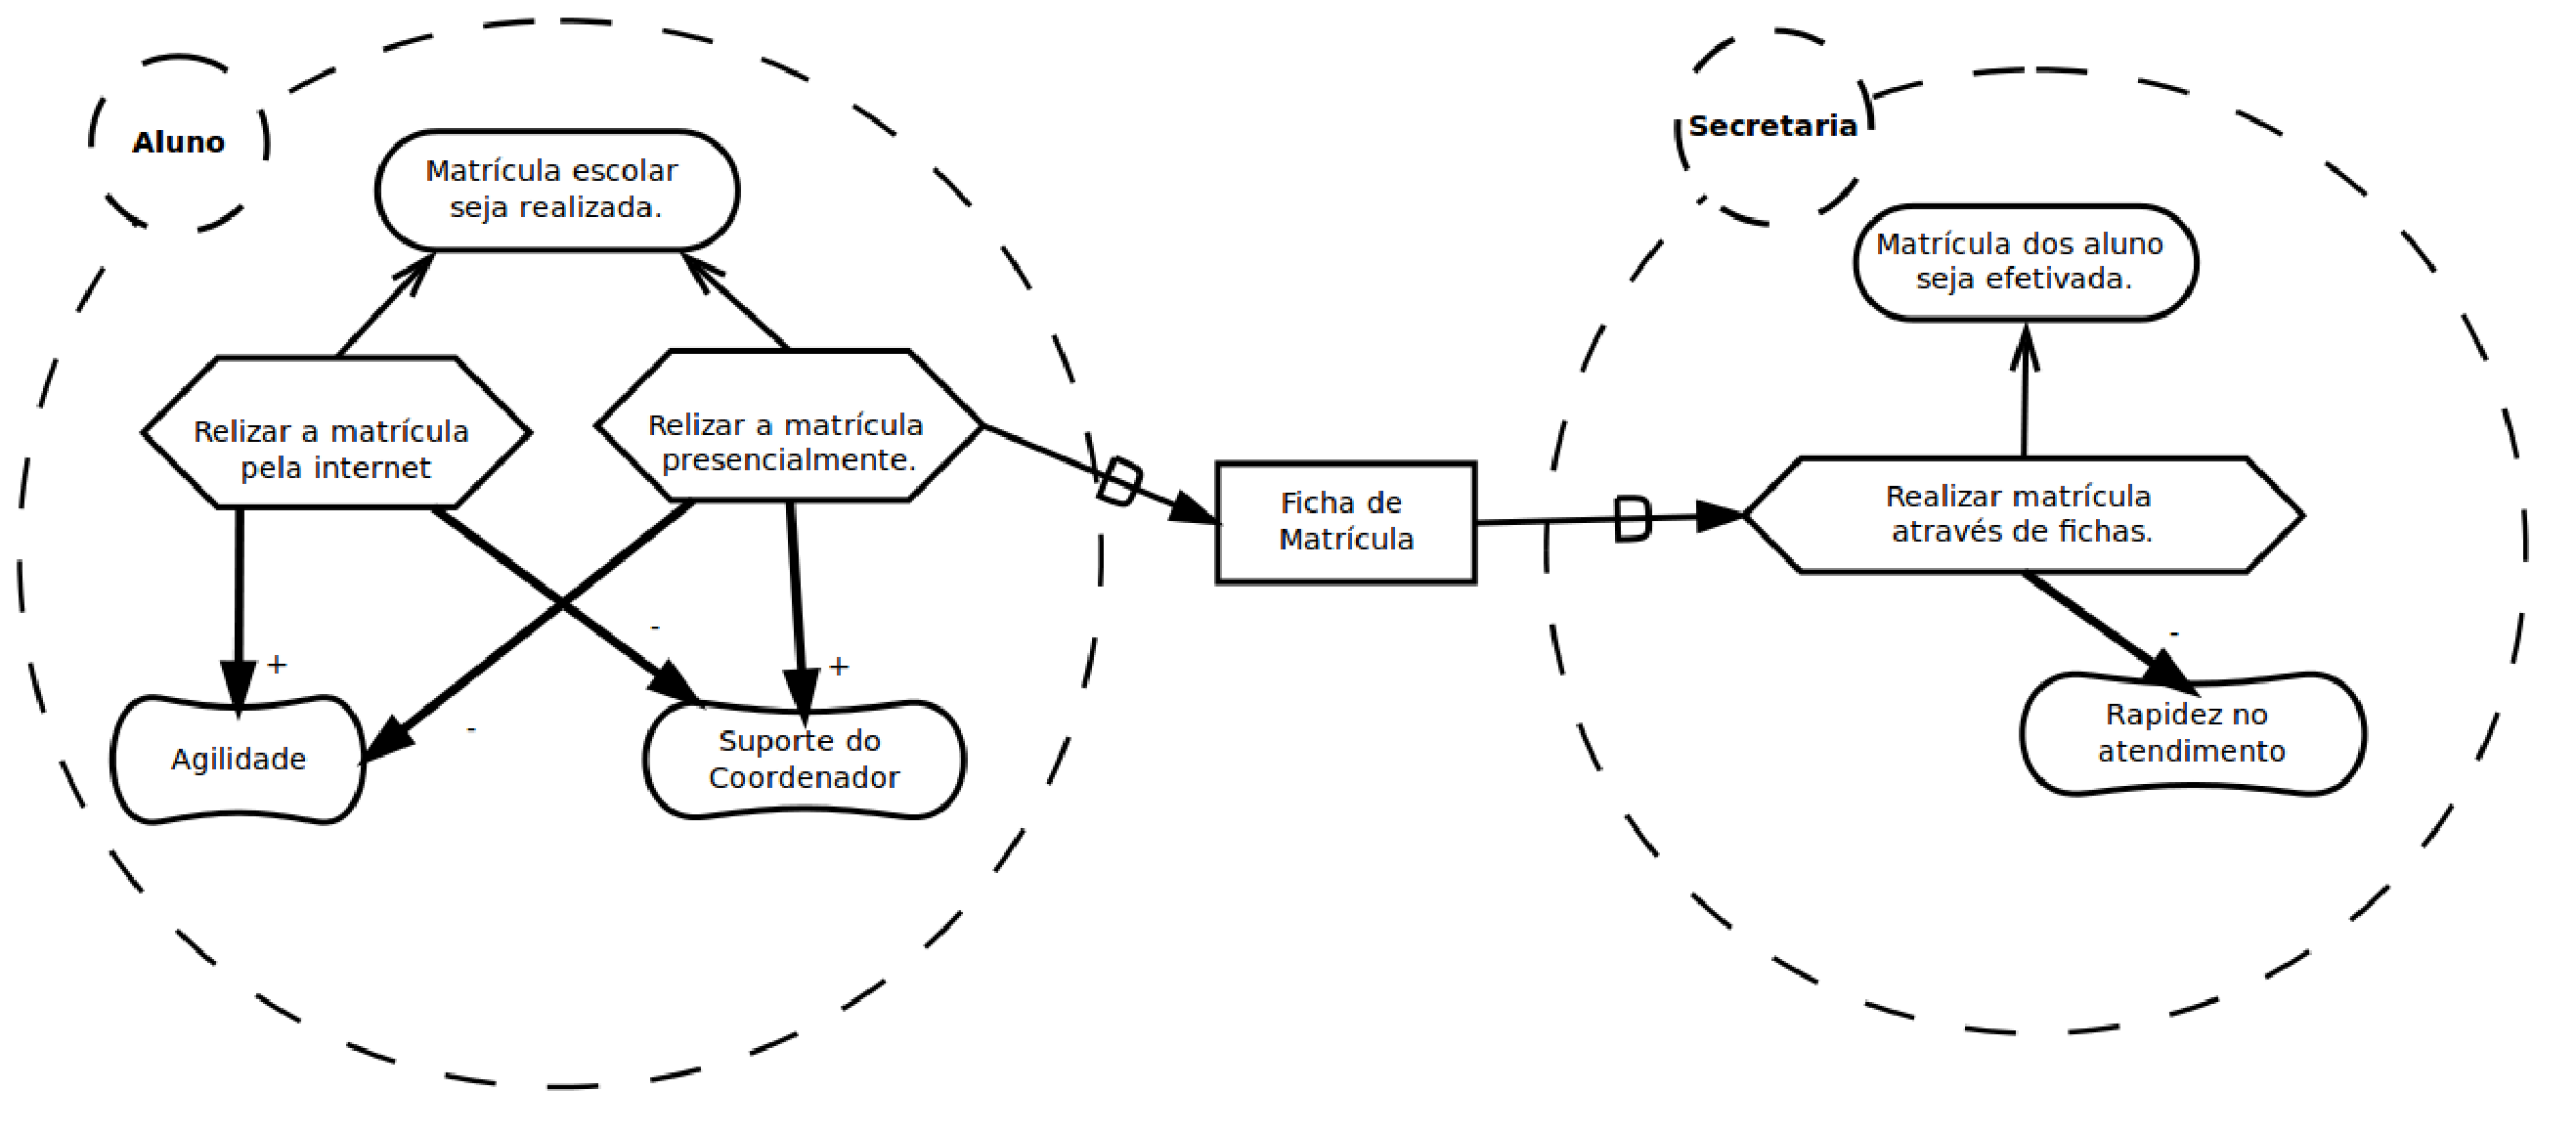
\includegraphics[width=1.1\textwidth]{exemplo-istar}
\caption{Aplicação do Framework I*} 
\label{exemplo-istar}
\end{figure}
 
A modelagem social é bastante flexível. Ela pode ser utilizada em diversos contextos, a metodologia ágil é um bom exemplo. Através de um estudo de caso, foi demonstrado que a utilização do framework I* enriquece a especificação das histórias de usuário \cite{jaqueira_2013}.

Utilizando a orientação a metas é possível determinar a origem dos conceitos existentes na especificação de requisitos. Para cada meta definida várias alternativas de solução devem ser determinadas. Ao longo da elicitação diversas validações são realizadas, assim requisitos inconsistentes expressadas pelo ator são identificados e removidos rapidamente \cite{zdra2013}.


\section{Grails: Groovy on Rails}
\label{grails_web}

O Grails é um framework para desenvolvimento de aplicações Web de alta produtividade, inspirado no Ruby on Rails, entretanto, utilizando linguagens como Java e Groovy. Este framework provê diferentes suportes e modelos
visando maior produtividade, extensibilidade, reusabilidade, portabilidade, confiabilidade, dentre outros critérios de qualidade. 	

O framework Grails oferece suporte baseado em bibliotecas Java bem estabelecidas no mercado, tais como: Hibernate, Maven, SiteMesh, Spring, dentre outros. Adicionalmente, o Grails pode ser integrado a qualquer biblioteca
Java através de plugins ou acesso direto. Todas as boas diretrizes do Java EE foram herdadas pelo Grails. 

Vale ressaltar que, segundo \cite{smith2009}, o Grails faz parte da próxima geração de frameworks de desenvolvimento Web baseados em Java, oferecendo ao desenvolvedor a possibilidade de obter, dentre outras vantagens, uma alta produtividade e reusabilidade. O Grails pode ser estendido por meio de plugins. No site oficial\footnote{$http://grails.org/plugins$} existem mais de mil opções, que oferecem serviços de segurança, teste, melhoria no desempenho, requisições AJAX, entre outros.

Para o aumento da produtividade, o Grails permite a codificação através do Groovy. O Groovy é uma linguagem dinâmica com sintaxe semelhante ao Java, compila para \textit{bytecodes} e executa na JVM. Apesar de semelhante, a sintaxe do Groovy é mais flexível e poderosa do que a sintaxe do Java. Permitindo a construção, desde simples \textit{shell scripts} a até aplicações robustas com milhares de linhas de código \cite{bashar2009}.   

A estrutura oferecida pelo Grails procura ser simples e consistente no que se refere ao uso de frameworks e bibliotecas já consolidadas no mercado. O desenvolvedor pode-se concentrar nas regras de negócio e em aspectos
específicos do domínio cognitivo de interesse, uma vez que detalhes técnicos de configuração, os quais demandam um tempo considerável de desenvolvimento em frameworks tradicionais, são altamente facilitados no ambiente de desenvolvimento do Grails.

No intuito de prover uma maior compreensão quanto a execução de uma aplicação em Grails, a Figura \ref{execucao-grails} ilustra os principais elementos envolvidos no funcionamento do núcleo da aplicação.

\graphicspath{{figuras/}}
\begin{figure}[H]
\centering
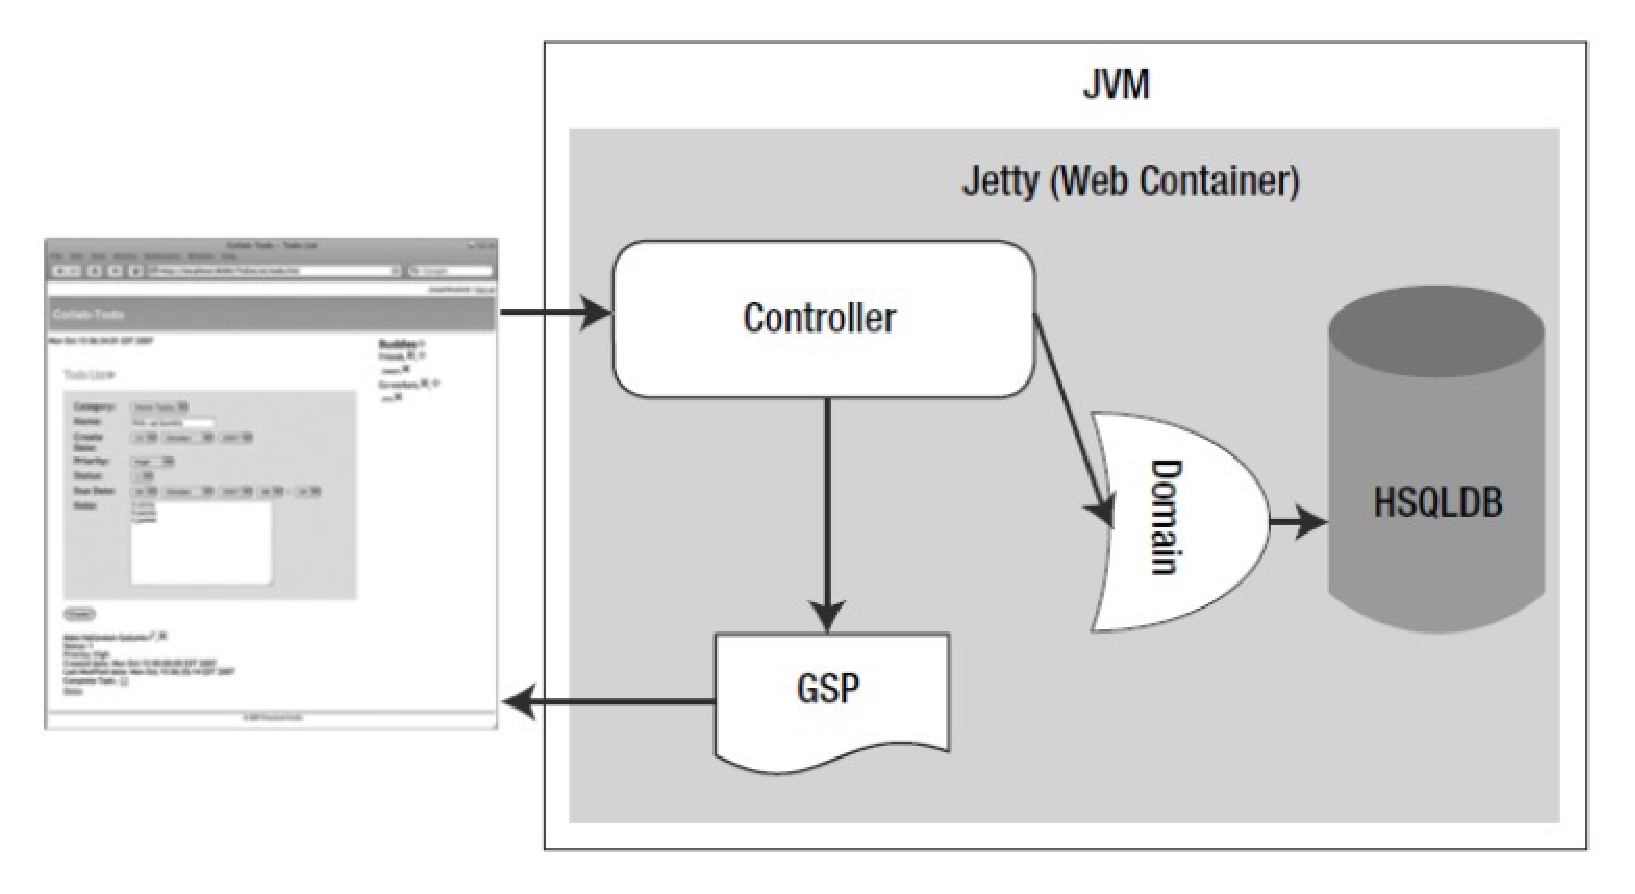
\includegraphics[width=1.0\textwidth]{execucao-grails}
\caption{Visão de Execução do Grails}{Extraído de \cite{juddbeginning2008}} 
\label{execucao-grails}
\end{figure}

Inicialmente, é realizada uma requisição através do browser para um servidor Web Jetty (i.e. Apache Tomcat ou outro). A controladora recebe e trata essa requisição podendo resolvê-la sozinha ou requisitando os serviços de
alguma classe de domínio. Todas as classes contidas no domínio são persistidas utilizando o framework GORM. Assim, padrões como DAO ou \textit{Repositor} não precisam ser utilizados. Quando a controladora finaliza a operação requisitada, ela envia o resultado para o GSP, que representa a view que irá renderizar o HTML, o qual será retornado para o browser que o havia requerido.

\subsection{Arquitetura}

O Grails possui características semelhantes ao Ruby on Rails (ROR). Dada a complexidade dessa plataforma, vale destacar que o Grails, assim como o ROR, estabelece uma arquitetura própria, baseada, principalmente, nos componentes ilustrados na Figura \ref{arquitetura-grails}. 

\graphicspath{{figuras/}}
\begin{figure}[H]
\centering
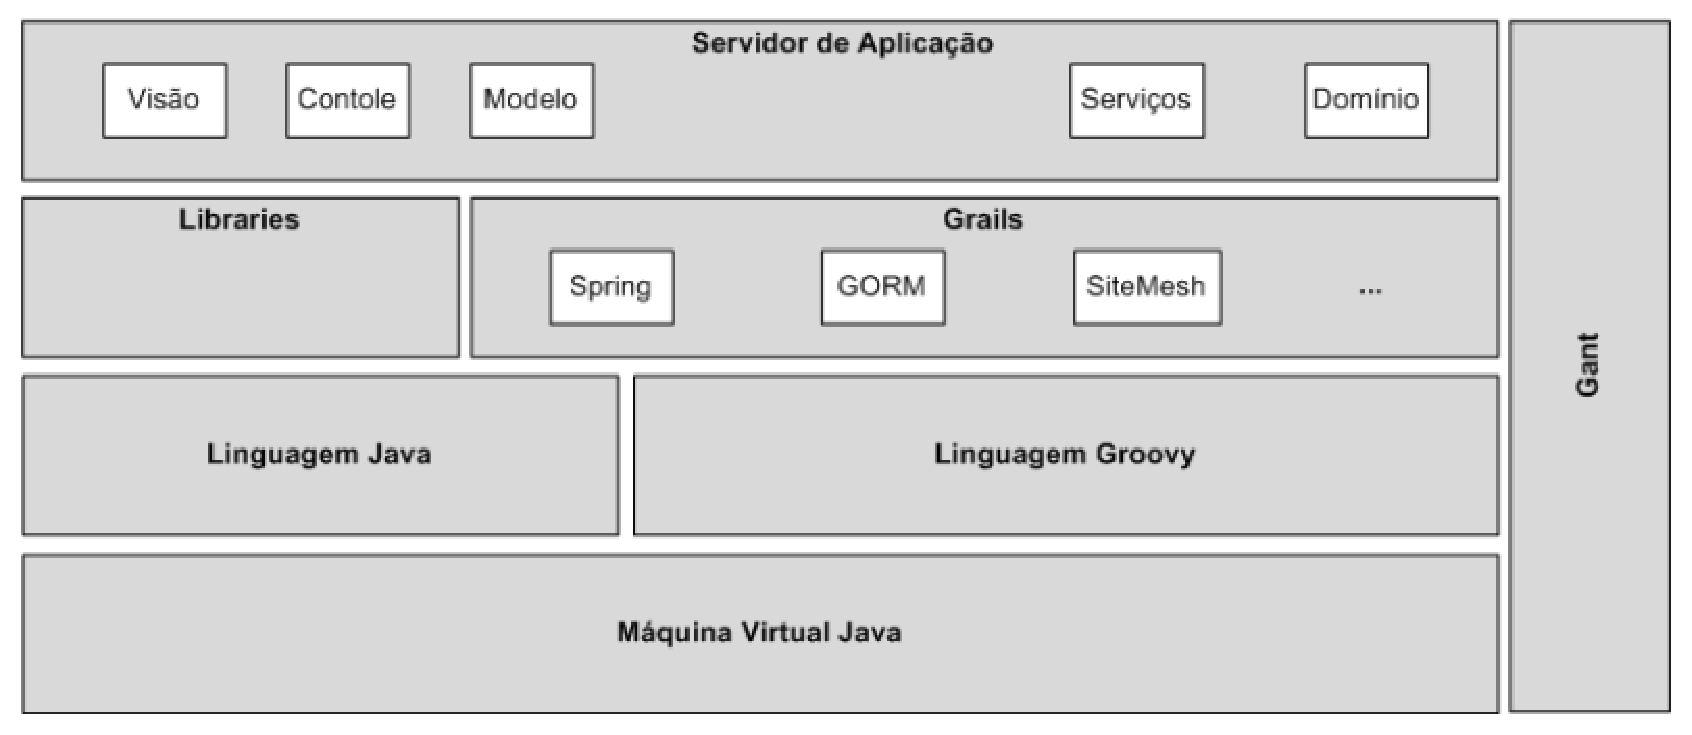
\includegraphics[width=1.0\textwidth]{arquitetura-grails}
\caption{Arquitetura do Grails}{Adaptação de \cite{juddbeginning2008}} 
\label{arquitetura-grails}
\end{figure}

Como apresentado, a base do Grails é a Máquina Virtual Java (JVM), programa que carrega e executa as aplicações Java, convertendo \textit{bytecodes} em código executável, compreendidos pela máquina. Acima da JVM são vistas duas linguagens, a linguagem Java e a linguagem Groovy. A separação entre a linguagem Java e a JVM deve-se à constante criação de novas bibliotecas para a plataforma.

O framework Grails provê compatibilidade com qualquer tipo de código escrito em Java. Sendo assim, caso um software legado em Java precise ser reaproveitado, o Grails é capaz de realizar esta tarefa através dos seus recursos sem maiores problemas. 

Na camada logo acima das linguagens, o núcleo do Grails é de fato encontrado, ele é composto de projetos \textit{open-source}, desenvolvidos pela indústria (ex. o framework Spring), oferecendo um conjunto de componentes facilmente integráveis à aplicação. Adicionalmente, permite ao desenvolvedor concentrar-se apenas nas regras de negócio, cabendo, por exemplo: (i) ao SiteMesh a definição de layouts reutilizáveis para páginas GSP ou JSP, e (ii) ao GORM prover elementos para definir relacionamentos entre classes de domínio. Outras bibliotecas construídas a partir de Groovy ou Java podem ser utilizadas sem problemas, seja código aberto ou proprietário.

A última camada da arquitetura interna do Grails é a de aplicação. É nesta camada que será implementada toda a aplicação do sistema (Classes de Domínio, Controladoras, Visões, dentre outros detalhes). Ressalta-se o uso do padrão arquitetural \textit{Model-View-Controller} (MVC), o qual facilita a organização e execução do sistema em desenvolvimento.

A fim de gerenciar os projetos e artefatos Grails, a arquitetura interna deste framework provê um componente chamado Gant. O Gant é um framework que gerencia \textit{builds}, utilizando a linguagem Groovy na criação de Scripts Apache Ant.

\section{Node.JS}

O Node.js é uma plataforma desenvolvida a partir da \textit{engine} JavaScript V8 da Google. Esta plataforma permite a construção de aplicações em rede escaláveis de forma trivial e produtiva. Para isto, oferece um modelo orientado a eventos assíncronos com um esquema de recursos \textit{non-blocking}, que o faz uma solução leve e eficiente para aplicações em tempo real com intenso uso de dados. Diferente de vários plataformas \textit{open-source}, o Node.js é fácil de inicializar e não requer recursos da máquina em excesso, como memória ou espaço de disco. 

Atualmente, existem várias tecnologias consolidadas para \textit{front-end} e \textit{back-end}. O papel do Node.js é oferecer uma interface consistente entre estas duas tecnologias. Apresenta-se na Figura \ref{atuacao-nodejs} um esquema exibindo onde o Node.js se encaixa no contexto de desenvolvimento de software.   

\graphicspath{{figuras/}}
\begin{figure}[H]
\centering
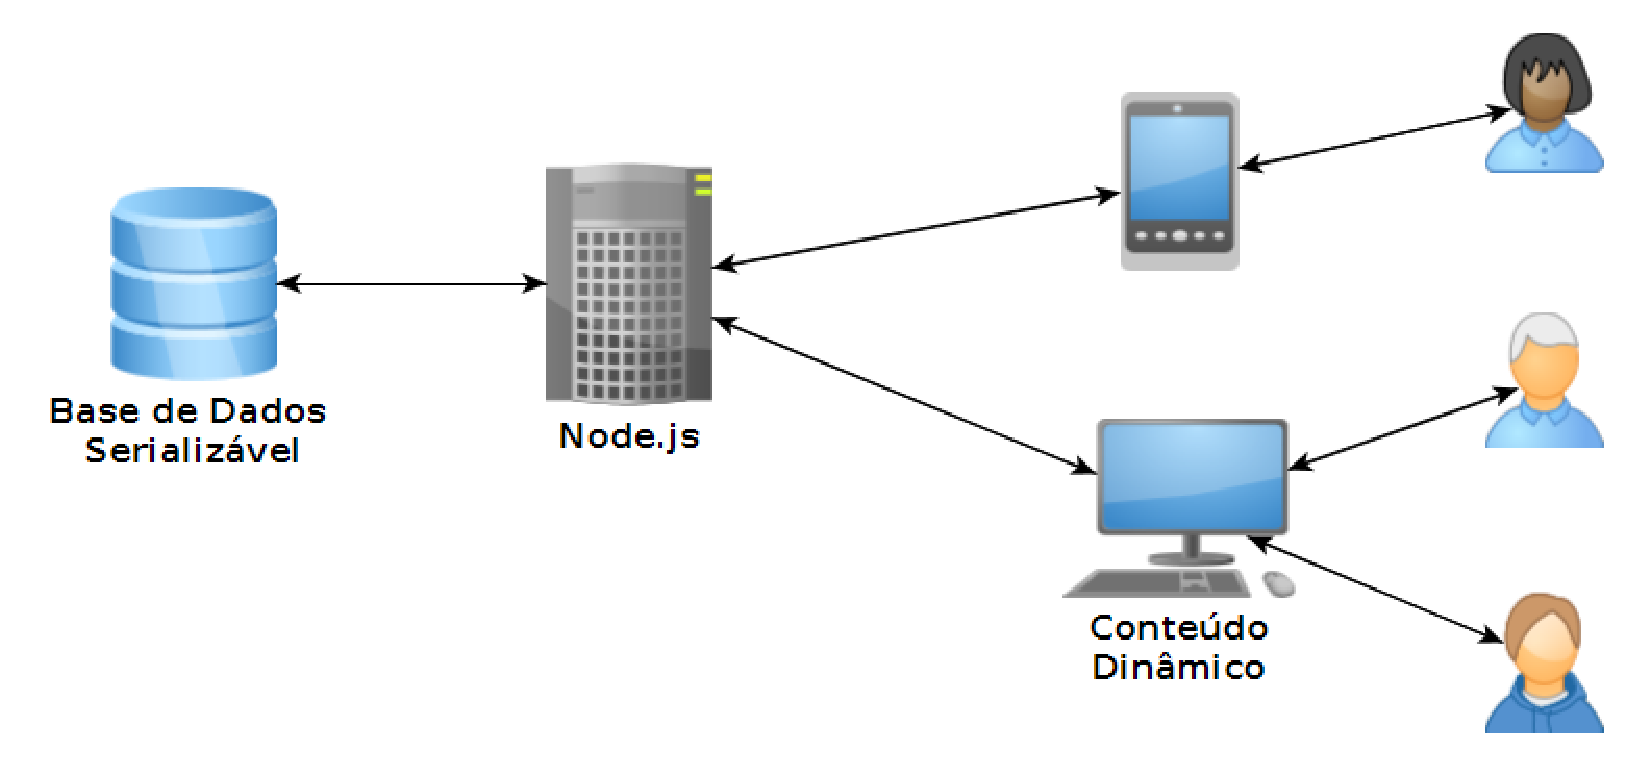
\includegraphics[width=1.0\textwidth]{atuacao-nodejs}
\caption{Atuação do Node.js}{Adaptação de \cite{wilson2013}} 
\label{atuacao-nodejs}
\end{figure}

O Node.js exerce seu trabalho através de um laço de eventos. O laço funciona da seguinte forma: (i) Carrega e executa o programa; (ii) inicializa o laço de eventos; (iii) espera algum evento ser disparado; (iv) executa os manipuladores de eventos; (v) finaliza o processo, se o mesmo estiver ocioso. Sempre que um evento ocorrer, o Node.js irá executar as \textit{callbacks} que estão escutando aquele evento. Apresenta-se na Figura \ref{laco-nodejs} o laço de eventos do Node.js.

\graphicspath{{figuras/}}
\begin{figure}[H]
\centering
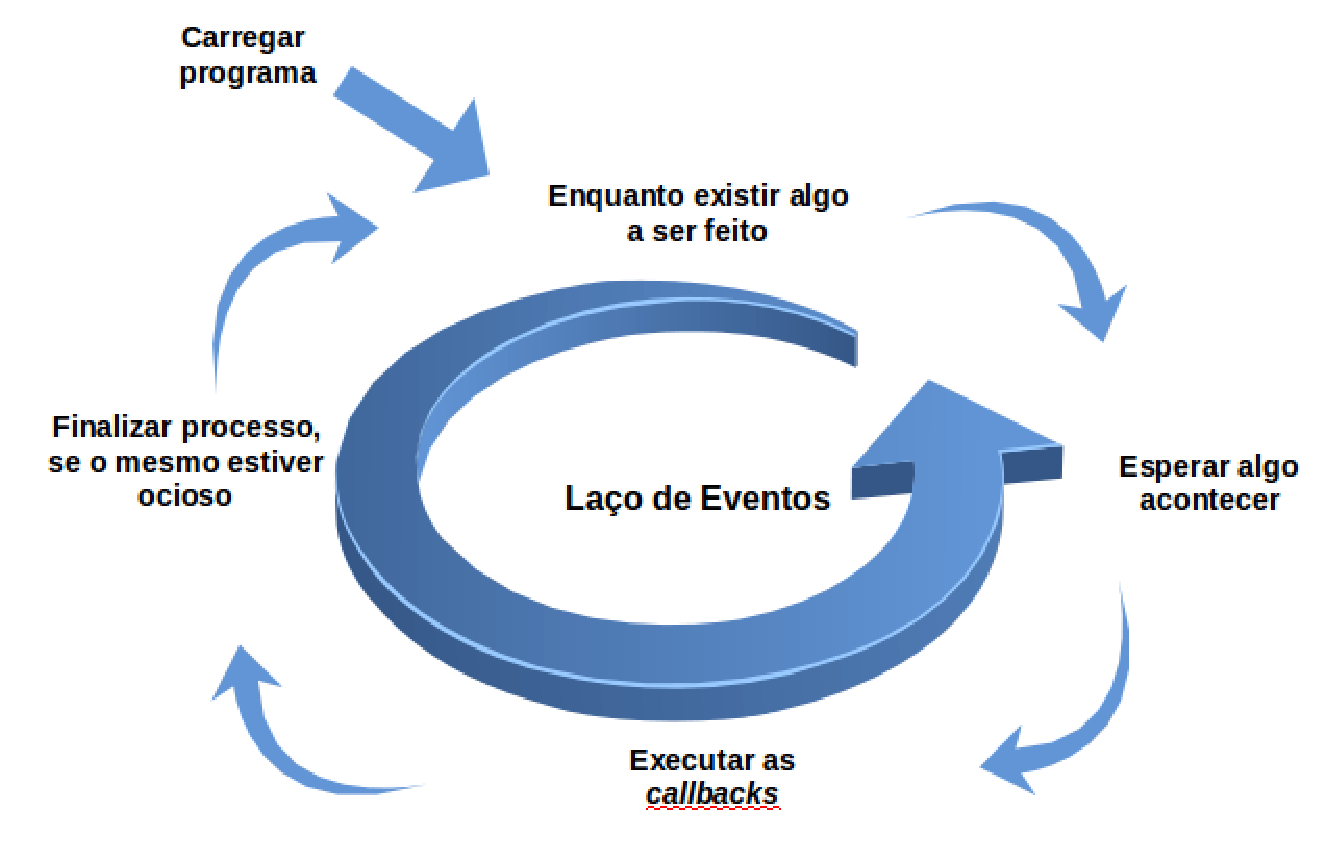
\includegraphics[width=1.0\textwidth]{laco-nodejs}
\caption{Laço de Eventos do Node.js}{Adaptação de \cite{wilson2013}} 
\label{laco-nodejs}
\end{figure}

As plataformas tradicionais que oferecem serviços web exigem que para cada requisição, uma \textit{thread} seja criada. Cada nova \textit{thread} consome uma quantidade específica de memória RAM. Uma aplicação contendo um alto fluxo de requisições necessitaria de uma infraestrutura consistente para funcionar adequadamente. O Node.js funciona de uma forma diferente, ele opera em uma única \textit{thread} utilizando chamadas de entrada e saída não bloqueantes. Assim, permitindo milhares de requisições concorrentes e poupando, consideravelmente, o consumo dos recursos computacionais.

\section{Twitter Bootstrap}

A partir da necessidade de padronizar as ferramentas e bibliotecas \textit{front-end} da empresa Twitter, Mark Otto e Jacob Thornton desenvolveram um framework \textit{open source} chamado Bootstrap. Este framework oferece um projeto baseado em arquivos CSS, plugins JavaScript e ícones que permitem o desenvolvimento de interfaces gráficas responsivas. Através da ferramenta de customização disponível no site oficial\footnote{$http://getbootstrap.com/customize/$} é possível selecionar quais componentes CSS e funcionalidades JavaScript irão fazer parte da aplicação.

Apresenta-se a estrutura de arquivos do Bootstrap na Figura \ref{estrutura-bootstrap}.

\graphicspath{{figuras/}}
\begin{figure}[H]
\centering
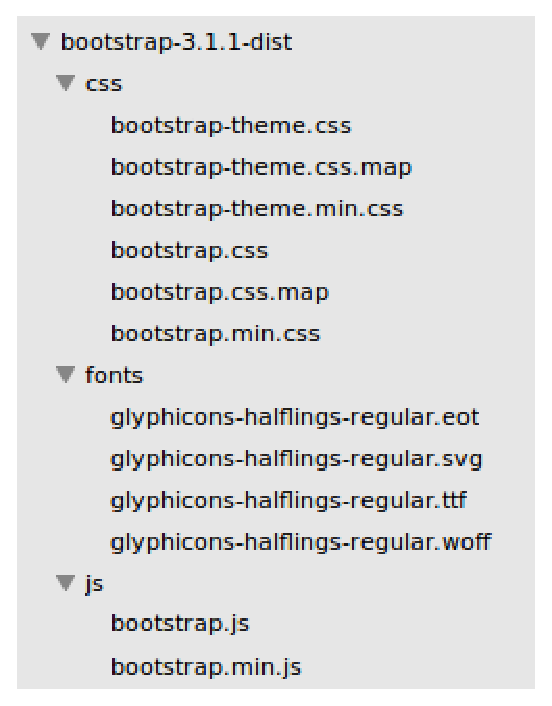
\includegraphics[width=0.5\textwidth]{estrutura-bootstrap}
\caption{Estrutura de Diretórios do Bootstrap}
\label{estrutura-bootstrap}
\end{figure}

O Bootstrap é compatível com as últimas versões de diversos navegadores, tais como Internet Explorer, Mozilla Firefox, Google Chrome e Opera. Navegadores de dispositivos móveis também oferecem suporte ao Bootstrap. A partir da versão 2.0, o suporte ao \textit{design} responsivo das páginas web foi integrado ao framework.

Para utilizar o Bootstrap, basta baixar o código fonte e adicioná-lo na página HTML. Outra opção seria referenciar uma CDN\footnote{Content Delivery Network ou Rede de Fornecimento de Conteúdo} confiável na página HTML. Esta segunda opção é viável quando não é necessário customizar os arquivos fontes. Ao término da instalação, o desenvolvedor adquire uma lista de componentes web, tais como, botões, tabelas, menus prontos para serem utilizados. 

Na Figura \ref{uso-bootstrap}, apresenta-se um exemplo enfatizando o uso do Bootstrap. Neste exemplo utiliza-se alguns componentes interessantes tais como, \textit{navbar}, \textit{jumbotron} e o sistema de \textit{grid}.

\graphicspath{{figuras/}}
\begin{figure}[H]
\centering
\includegraphics[width=1.0\textwidth]{uso-bootstrap}
\caption{Aplicação do Twiiter Bootstrap}{Adaptação de $http://bootstrapdocs.com/v3.1.1/docs/examples/jumbotron/$}
\label{uso-bootstrap}
\end{figure}
  











